\chapter{Estado del Arte}\label{chapter:state-of-the-art}
    Este capítulo proporciona una panorámica del estado de las investigaciones relacionadas con la generación de Estados del Arte. Que a efectos de esta investigación se entiende como un resumen de múltiples documentos relacionados con un tema. Por ello se comienza por analizar los más recientes avances acerca de la generación de resúmenes automáticos así como de las las herramientas necesarias para la resolución de problemas específicos que enfrentan los enfoques con los que se generan dichos resúmenes.

\section{Procesado de Documentos para facilitar la investigación científica}
Durante el estudio del estado del arte se hizo evidente una ausencia de investigaciones recientes que se puedan vincular directamente con el objetivo específico de esta investigación, no obstante trabajos como el presentado por (Portenoy, J. y West, J.D., 2020)[\cite{portenoy2020constructing}] han intentado resolver el problema de la construcción de un resumen de trabajos relacionados con un documento, basados en una red de citaciones combinada con elementos extraídos del texto, donde la selección de los datos se realiza mediante un agrupamiento del corpus utilizado. (Marshall et al., 2017)[\cite{marshall}] 
proponen un modelo de generación de resultados provenientes de revistas médicas mediante un clasificador que utiliza un grupo de categorías descriptivas obtenidas mediante técnicas de procesamiento de lenguaje natural. Sin embargo estas investigaciones dejan en evidencia la ausencia tanto de investigaciones como de corpus de fácil acceso para la evaluación de los modelos relacionados con esta tarea.

\section{Sistemas de generación automática de resúmenes utilizando enfoques híbridos}

Un enfoque híbrido combina tanto las aproximaciones extractivas como abstractivas en el proceso de resumen de texto. La arquitectura típica  de un generador de resúmenes automáticos de textos híbrido se muestra en la Figura 1 y consta comúnmente de las siguientes fases:

\begin{enumerate}
    \item Preprocesamiento
    \item Extracción de oraciones (fase extractiva): Extraer las oraciones clave del texto de entrada. (Wang et al., 2017)[\cite{Wang}]
    \item Generación del resumen (fase abstractiva): Generar el resumen final a partir de la aplicación de métodos abstractivos a las oraciones previamente extraídas.
    \item Post procesamiento: Verificar que las oraciones generadas sean válidas y se ajusten al formato deseado.
\end{enumerate}

\begin{figure}[H]    
    \centering
    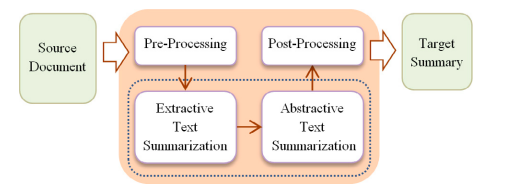
\includegraphics[scale = 1]{Figures/hybrid.png}
    \caption*{Figura 1: Estructura de un generador de resúmenes híbrido}
\end{figure}

En la propuesta de (Rasim et al., 2019)[\cite{cosum}] se utiliza un modelo de dos etapas que combina técnicas de \emph{clustering} y optimización. En la primera etapa, se aplica el método de \emph{k-means} para agrupar las oraciones y descubrir múltiples temas en el texto. En la segunda etapa, se implementa un modelo de optimización para la selección de oraciones destacadas de los clusters. Otro enfoque interesante es el de (Ghadimi y Beigy, 2022)[\cite{hybrid-llm}] que inicialmente construye un resumen extractivo a partir de varios documentos de entrada y luego lo utiliza para generar el resumen abstractivo. La gestión de la información redundante, un problema global en el campo de la síntesis de múltiples documentos, se aborda en la primera etapa donde se utilizan similitudes basadas en BERT[\cite{BERT}] para calcular la redundancia de los documentos.

La incorporación de Grandes Modelos de Lenguaje (LLM, por sus siglas en inglés) ha revolucionado el campo de procesamiento de lenguaje natural (NLP, por sus siglas en inglés), abriendo nuevas posibilidades y elevando el rendimiento en diversas tareas. Entre ellas, la condensación de textos. En investigaciones como la realizada por (Basyal et al, 2023)[\cite{basyal2023text}] se observa el excepcional desempeño de los modelos de lenguaje, principalmente el modelo \emph{text-davinci-003} de OpenAI[\cite{openai}]. No obstante se aclara que los modelos con los que fue comparado son significativamente más peque\~nos y se sugiere hacer uso de sus versiones más complejas.

\section{Topic Modeling}

    El análisis de texto ha experimentado avances significativos en las últimas décadas y entre las técnicas más destacadas se encuentra el Modelado de Temas (\emph{Topic Modeling}). Esta metodología, anclada en la minería de texto y el procesamiento de lenguaje natural, ha emergido como una herramienta escencial para descubrir patrones subyacentes y estructuras temáticas en grandes conjuntos de documentos. El Modelado de Temas se adentra en la complejidad de los datos textuales, permitiendo la identificación automática y la organización de temas latentes presentes en un corpus[\cite{lda2003}].

    El uso de modelos basados en la arquitectura \emph{encoder-decoder} se ha usado para la generación de algoritmos de \emph{Topic Modeling }tanto para textos cortos[\cite{neuraltm}] como para textos extensos[\cite{tminemb}]. En todos los casos, han mejorado comparado con los resultados generados por herramientas más tradicionales y ampliamente usados como \emph{Latent Dirichlet Analysis (LDA)}[\cite{lda2003}].  

    Angelov (2020)[\cite{angelov2020top2vec}] presenta un nuevo modelo que utiliza \emph{embeddings} semánticos para identificar temas sin requerir parámetros predefinidos ni listas personalizadas. A diferencia de los métodos tradicionales, este captura la semántica tanto de palabras como de documentos, y arroja resultados más informativos y representativos en los experimentos desarrollados por el autor.

    \subsection{Clustering}
    Utilizando una representación en vectores de la información a través de \emph{embeddings} de texto (Sia et al. 2020)[\cite{sia2020tired}] presenta evaluaciones comparativas para la combinación de diferentes \emph{embeddings} de palabras y algoritmos de agrupamiento al tiempo que analiza el rendimiento bajo reducción de dimensionalidad con PCA\footnote{El Análisis de Componentes Principales, PCA, es una herramienta de reducción de dimensiones que se utiliza para reducir un gran conjunto de variables en uno menor pero que contenga la mayor parte de la información relevante}. En algunos casos ha tenido resultados tan sólidos como los obtenidos por modelos de temas clásicos[\cite{sia2020tiredResults}], pero con menor tiempo de ejecución y complejidad computacional. 
    Por esta línea, se encuentra también \emph{BERTopic}[\cite{bertopic}] que hace una primera representación de los documentos como \emph{text embeddings}, realiza un agrupamiento en el espacio de los vectores generados y construye los títulos de los temas utilizando un sistema de representación categórica a través de una tabla \emph{TF-IDF}\footnote{TF-IDF (\emph{Term Frequency-Inverse Document Frequency}) es una técnica de ponderación que evalúa la importancia relativa de una palabra en un documento dentro de un conjunto de documentos, considerando tanto la frecuencia de la palabra en el documento como su rareza en el conjunto.}.

\section{Embeddings de texto}
    En la exploración de \emph{embeddings} contextuales, según detalla Liu et al. (2020)[\cite{liu2020survey}], el enfoque se centra en asignar representaciones a palabras basadas en su contexto, al tiempo que captura sus diversos usos y codifica conocimientos transferibles entre idiomas. Su estudio profundiza en varios aspectos, incluidos los modelos existentes de \emph{embeddings} contextuales, el preentrenamiento políglota entre idiomas y la aplicación de \emph{embeddings} contextuales en tareas posteriores.

    Huang et al. (2020)[\cite{Huang_2020}] destacan las ventajas de la aplicación de estos al ámbito de los sistemas de búsqueda, especialmente en redes sociales como Facebook. Los autores presentan un marco de recuperación basado en \emph{embeddings} (\textbbf{EBR}) y un marco de \emph{embeddings} unificado para la búsqueda personalizada, en el que exponen sus experiencias y optimizaciones para mejoras integrales en el sistema. Su trabajo sobre \emph{EBR} en la búsqueda de Facebook presentan ganancias significativas en cuanto a métricas evaluadas en experimentos en línea.

    Reimers et al. (2022)[\cite{reimers2019sentencebert}] abordan la sobrecarga computacional asociada con modelos como \emph{BERT} y \emph{RoBERTa} en tareas de regresión de pares de oraciones. Introducen \emph{Sentence-BERT} (\emph{SBERT}), una modificación de \emph{BERT} que utiliza estructuras de redes siamesas y tripletas para derivar \emph{embeddings} de oraciones semánticamente significativos. \emph{SBERT} reduce significativamente el esfuerzo computacional requerido para encontrar pares de oraciones similares, sin sacrificar la precisión. Su evaluación demuestra un rendimiento superior en tareas de similitud textual semántica (\emph{STS}) y tareas de transferencia en comparación con otros métodos de \emph{embedding} de oraciones de última generación.

    Gao et al. (2021)[\cite{gao2022simcse}] contribuyen al campo con \emph{SimCSE}, a partir de la presentación de modelos de aprendizaje contrastivo no supervisado y supervisado que mejoran significativamente los \emph{embeddings} de oraciones. Su enfoque, que utiliza \emph{dropout} como un mínimo aumento de datos, logra resultados destacados en tareas de similitud textual semántica (\emph{STS}). El enfoque supervisado, que incorpora pares anotados, mejora aún más la correlación. Y destaca la efectividad del objetivo de aprendizaje contrastivo tanto en la regularización como en la alineación de los \emph{embeddings} preentrenados.

    (Muenninghoff et al. 2023)[\cite{muennighoff2023mteb}] presentan el \emph{Massive Text Embedding Benchmark} (\emph{MTEB}), una iniciativa que abarca ocho tareas de \emph{embedding}, 58 conjuntos de datos y 112 idiomas. A través de la evaluación de 33 modelos en \emph{MTEB}, se establece el benchmark más completo hasta la fecha. Los resultados revelan que ningún método de \emph{embedding} de texto específico domina en todas las tareas, lo que sugiere que el campo aún no ha convergido hacia un método universal. \emph{MTEB} se presenta como una solución de código abierto y un ranking público [\cite{leaderboard}]. Este enfoque transparente y accesible contribuye a un mejor entendimiento y selección de modelos de \emph{embedding} de texto, lo cual supone el avance y la consolidación en este campo dinámico.

\section{Modelos de Lenguaje}
   
    La influencia revolucionaria de las arquitecturas de \emph{transformers}, introducida en \emph{`Attention is All You Need'} [\cite{attention}], ha sido crucial para los grandes modelos de lenguaje (LLM). Modelos como \emph{BERT}[\cite{BERT}] avanzaron en la comprensión bidireccional del contexto, mientras que la serie \emph{GPT}\emph{(Generative Pre-trained Transformer)}, especialmente \emph{GPT-3}[\cite{brown2020language}], con un modelo de 175 mil millones de parámetros y su sucesor \emph{GPT4}[\cite{openai2023gpt4}] se mantienen a la cabeza de la innovación y desempeño. Otros de los modelos a destacar son los presentados por \emph{MetaAI, LLaMA}(Feb. 2023)[\cite{llamapaper}] y \emph{LLaMA2}(Jul. 2023)[\cite{llamapaper2}], una colección de \emph{LLM} preentrenados y ajustados finamente que varían en escala desde 7 mil millones hasta 70 mil millones de parámetrosy que muestran resultados prometedores en comparación con otros modelos[\cite{metallama}]. 
    
    \subsection{Generación de resúmenes haciendo uso de LLM}

    En el trabajo de (Basyal et al. 2023)[\cite{basyal2023text}] se exploran técnicas de resumen de texto que utilizan \emph{LLM},entre las que se incluyen \emph{MPT-7b-instruct}[\cite{mpt}], \emph{falcon-7b-instruct}[\cite{falcon}] y \emph{OpenAI ChatGPT} \emph{text-davinci-003}[\cite{brown2020language}]. El modelo \emph{text-davinci-003} destaca como el más efectivo en diversas métricas de evaluación. Se realiza una comparación detallada en diferentes conjuntos de datos, como CNN, Daily Mail y XSum, que aportan valiosas percepciones sobre el rendimiento de los \emph{LLM} en entornos variados. 

    \subsection{Modelos de \emph{GPT4All}}

        \emph{GPT4All} es un ecosistema de software libre que ha publicado un grupo de \emph{LLM} basados en la arquitectura \emph{transformers}[\cite{attention}]. Los modelos \emph{GPT4All} son producto de la cuantización\footnote{Cuantizar es un proceso en el cual se reduce la precisión de los números en una red neuronal, disminuyendo así los requisitos de memoria y permitiendo que modelos grandes se ejecuten en dispositivos con recursos limitados. En este contexto, cuantizar facilita el uso de modelos \emph{GPT4All} en computadoras con menos capacidad de hardware} de redes neuronales, un proceso que reduce los requisitos de \emph{VRAM}\footnote{La memoria \emph{VRAM} (\emph{Video Random Access Memory}) es utilizada tratar los datos y las operaciones relacionadas con la tarjeta gráfica} para ejecutar un Decodificador Transformer de varios miles de millones de parámetros. A través de algoritmos de cuantización, estos modelos pueden ser adaptados para poder ser utilizados con un hardware moderado[\cite{webgpt4all}].
        
        Entre los modelos soportados se encuentran\footnote{La cantidad de parámetros especificada se refiere a los modelos cuantizados disponibles en la web de \emph{GPT4All}}:

        \begin{enumerate}
            \item \emph{Falcon} (7 mil millones de parámetros)~[\cite{falcon}]
            \item \emph{LLaMA} (7 - 13 mil millones de parámetros)~[\cite{llama}]
            \item \emph{MPT} (7 mil millones de parámetros)~[\cite{mpt}]
            \item \emph{GPT-J} (6 mil millones de parámetros)~[\cite{gptj}]
        \end{enumerate}

